\lab{Invertible Affine Transformations and Linear Systems}{Invertible Affine Transformations and Linear Systems}
\label{lab:ChangeBasis}
\objective{Apply affine transformations to a set of vectors in $\mathbb{R}^2$ and solve linear systems.}

\section*{Linear transformations in $\mathbb{R}^2$}
\subsection*{Dilations}
A \emph{dilation} of the vector space rescales the vectors. 
Graphically, a dilation stretches or compresses the space. 
A linear transformation is a dilation if and only if its matrix representation is diagonal, so in particular all Type II elementary matrices are dilations. 
The matrix $\begin{pmatrix}
1.5 & 0\\
0 & 1.5 \end{pmatrix}$ corresponds to the dilation in Figure \ref{fig:dilation}.
\begin{figure}
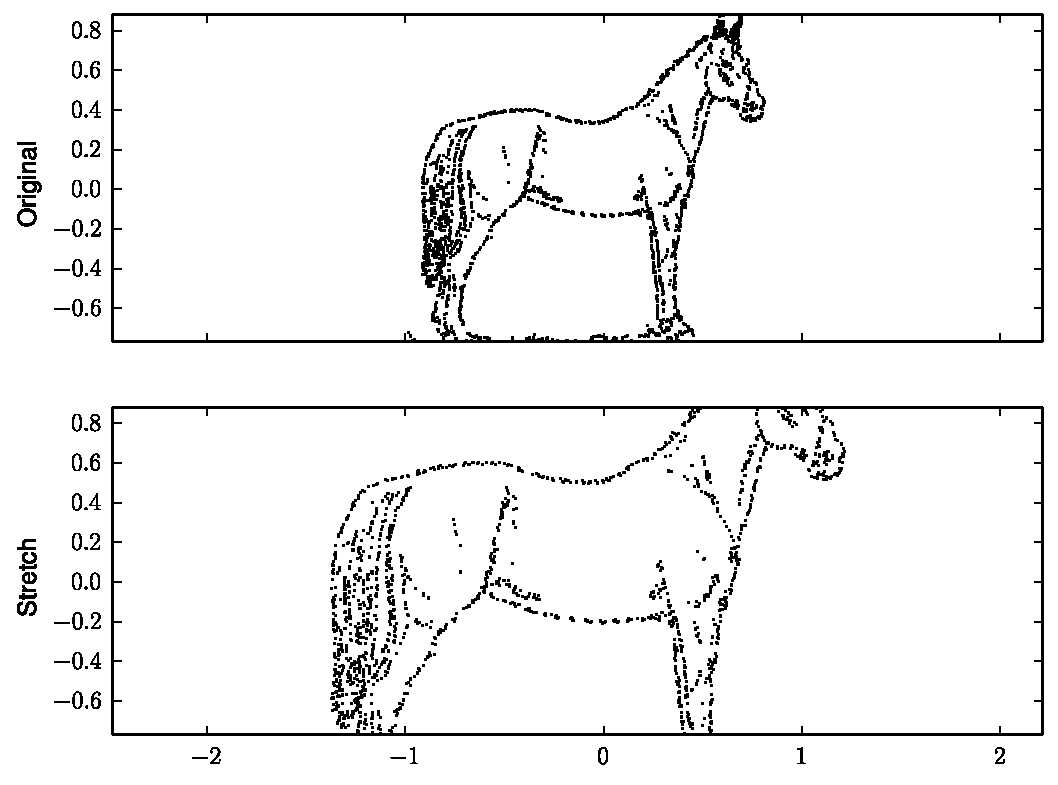
\includegraphics[width=\textwidth]{stretch.pdf}
\caption{An example of a dilation. 
The top image was stretched by a factor of $1.5$ in all directions, producing the bottom image.}
\label{fig:dilation}
\end{figure}

\begin{problem}\label{prob:dilation}
Write a function that accepts an array of points and an array giving the stretching factors in each direction. 
Your function should return the dilated points. 
Hint: To check your work, plot the original points and their images under the transformation using the function \li{plotOldNew()} defined below.
\begin{lstlisting}
import numpy as np
from matplotlib import pyplot as plt

def plotOldNew(old, new):
    '''Inputs:
    new -- a (2,n) numpy array containing x-coordinates on the 
            first row and y-coordinates on the second row.
    old -- a (2,n) numpy array containing x-coordinates on the first
            row and y-coordinates on the second row.
    '''
            
    plt.subplot(2, 1, 1)
    plt.scatter(old[0], old[1])
    plt.axis('equal')
    plt.subplot(2, 1, 2)
    plt.scatter(new[0], new[1])
    plt.show()
\end{lstlisting}
\end{problem}

\subsection*{Rotations}
A second type of linear transformation is to rotate vectors around the origin. 
A rotation of $\theta$ radians counterclockwise corresponds to the matrix $\begin{pmatrix}
\cos(\theta) & -\sin(\theta) \\
\sin(\theta) & \cos(\theta)
\end{pmatrix}.$ 
When $\theta = \pi/3$ we get the rotation matrix illustrated in Figure \ref{fig:rotate}.

\begin{figure}
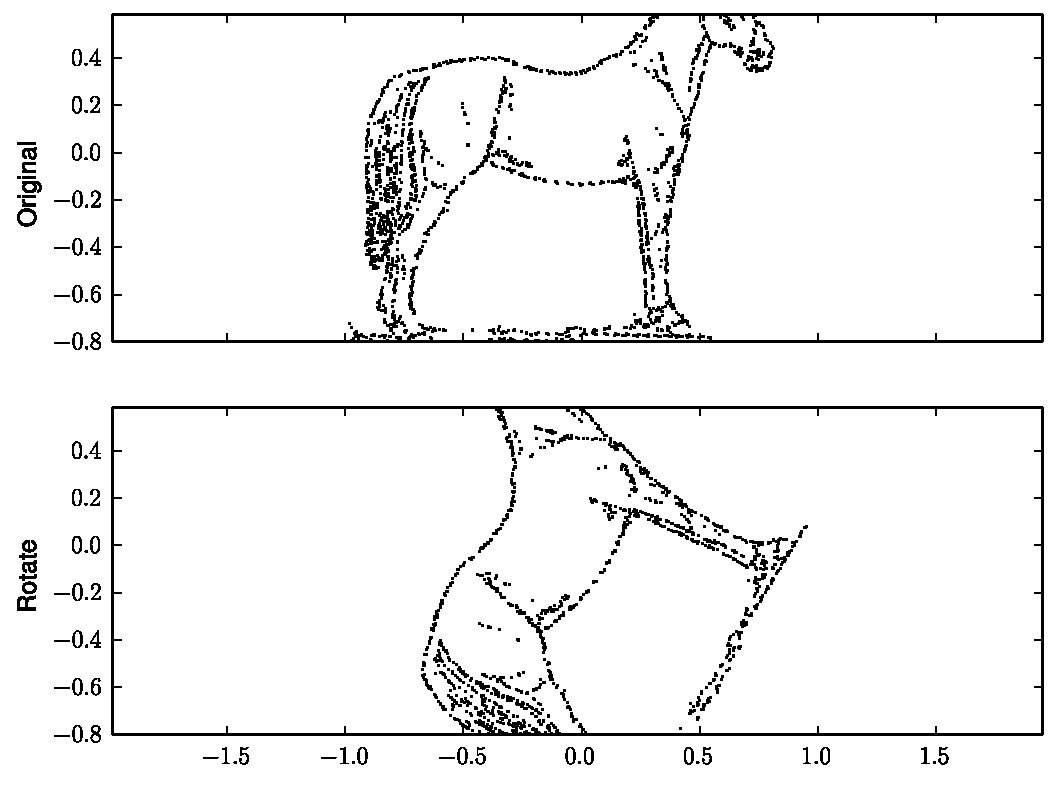
\includegraphics[width=\textwidth]{rotate.pdf}
\caption{An example of a rotation.
The top image was rotated by $\pi/3$, producing the bottom image.}
\label{fig:rotate}
\end{figure}

\begin{problem}
 Write a function that accepts an array of points and the angle of rotation (in radians). 
 Your function should return the rotated points. 
 Hint: To check your work, plot the original points and their images under the transformation using the function \li{plotOldNew()} defined in Problem \ref{prob:dilation}.
\end{problem}

\subsection*{Shears}

\begin{figure}
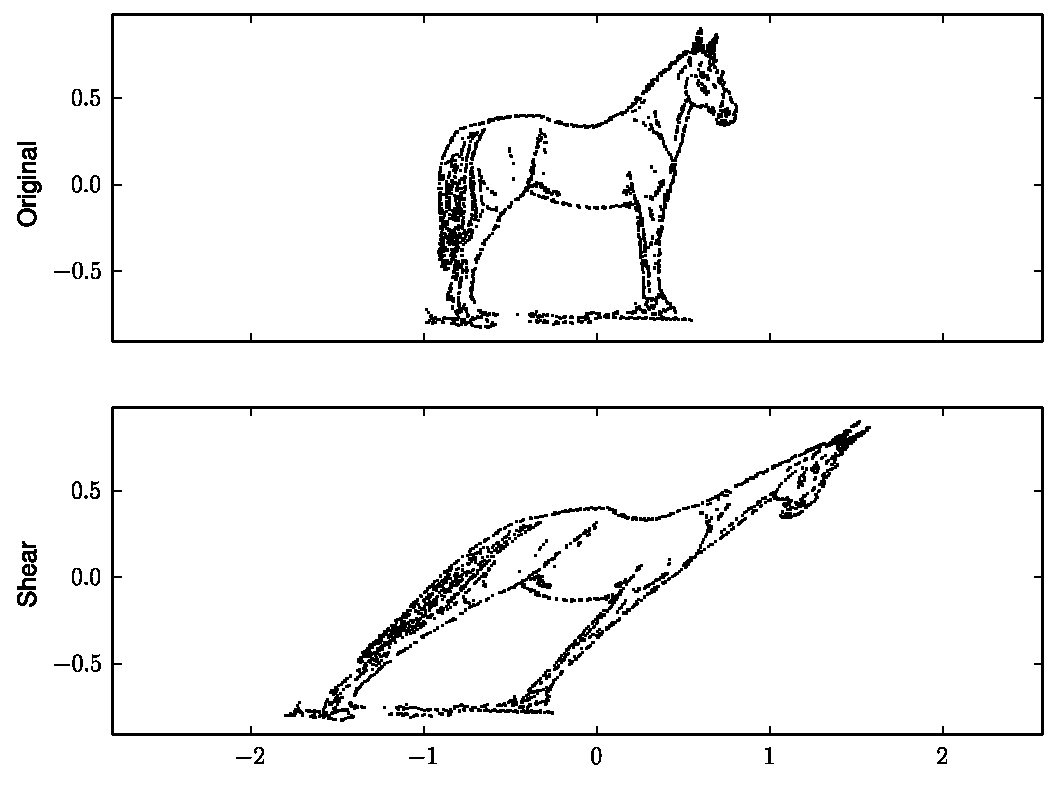
\includegraphics[width=\textwidth]{shear.pdf}
\caption{An example of a shear.
The top image was sheared horizontally to produce the bottom image.}
\label{fig:shear}
\end{figure}

A third type of linear transformation is a \emph{shear}, which ``slants'' a set of vectors. 
The corresponding matrix is a Type III elementary matrix. 
A horizontal shear has the form $\begin{pmatrix}
1 & c \\
0 & 1
\end{pmatrix}$ and a vertical skew has the form $
 \begin{pmatrix}
1 & 0 \\
c & 1
\end{pmatrix}
$. 
Notice that horizontal skews fix the $y$-coordinate of a vector while vertical skews fix the $x$-coordinate. 
The horizontal shear in Figure \ref{fig:shear} corresponds to the matrix $\begin{pmatrix}
1 & 1.02 \\
0 & 1
\end{pmatrix}
$.


\begin{problem}[Optional]
Write a function that accepts an array of points, a floating point argument that indicates the shearing amount, and an integer argument that indicates the direction of the shear (0 for horizontal, 1 for vertical). 
Your function should return the sheared points. 
Hint: To check your work, plot the original points and their images under the transformation using the function \li{plotOldNew()} defined in Problem \ref{prob:dilation}.
\end{problem}

\subsection*{Reflections}

\begin{figure}
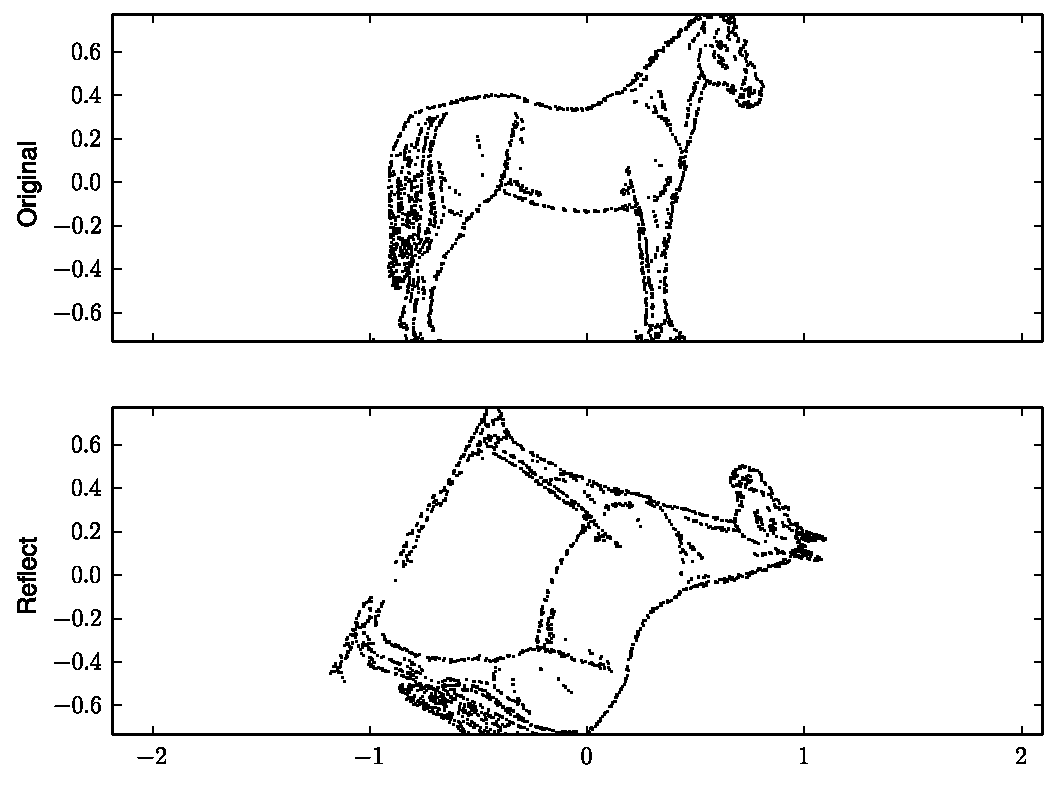
\includegraphics[width=\textwidth]{reflect.pdf}
\caption{An example of a reflection. 
The top image was reflected about the line $y = (1/\sqrt{3})x$, producing the bottom image.}
\label{fig:reflect}
\end{figure}
A fourth type of linear transformation is reflections about a line, also called \emph{Householder transformations}. 
Reflecting about a line spanned by $(l_1, l_2)$ corresponds to the matrix
\[
\frac{1}{l_1^2 + l_2^2}
\begin{pmatrix}
l_1^2 - l_2^2 & 2l_1l_2 \\
2l_1l_2 & l_2^2 - l_1^2
\end{pmatrix}.
\]

For example, the line $y=x$ is spanned by $(1, 1)$. 
In this case the corresponding matrix $\begin{pmatrix}
0 & 1\\
1 & 0
\end{pmatrix}$ is a Type I elementary matrix, in fact the only one of size $2 \times 2$. 
As another example, the reflection in Figure \ref{fig:reflection} about the line $y = (1/\sqrt{3})x$ corresponds to the matrix $\frac{1}{4}\begin{pmatrix}
2 & 2\sqrt{3}\\
2\sqrt{3} & -2
\end{pmatrix}$.

\begin{problem}[Optional]
Write a function that accepts an array of points and a 1-D array describing the axis of reflection (in the notation above, this argument is $(l_1, l_2)$. 
Your function should return the reflected points. 
Hint: To check your work, plot the original points and their images under the transformation using the function \li{plotOldNew()} defined in Problem \ref{prob:dilation}.
\end{problem}

\subsection*{Composition of linear transformations}
Recall that composition of linear transformations corresponds to matrix multiplication. 
For example, if $S$ is a matrix representing a shear and $R$ is a matrix representing a rotation, then $RS$ represents a shear followed by a rotation.

In fact, any linear transformation of $\mathbb{R}^2$ is a composition of the transformations discussed in this lab. 
This is because reflections, dilations, and shears provide us with all the elementary matrices, and every matrix is a product of elementary matrices. 

\section*{Affine transformations}
\subsection*{Translations}

\begin{figure}
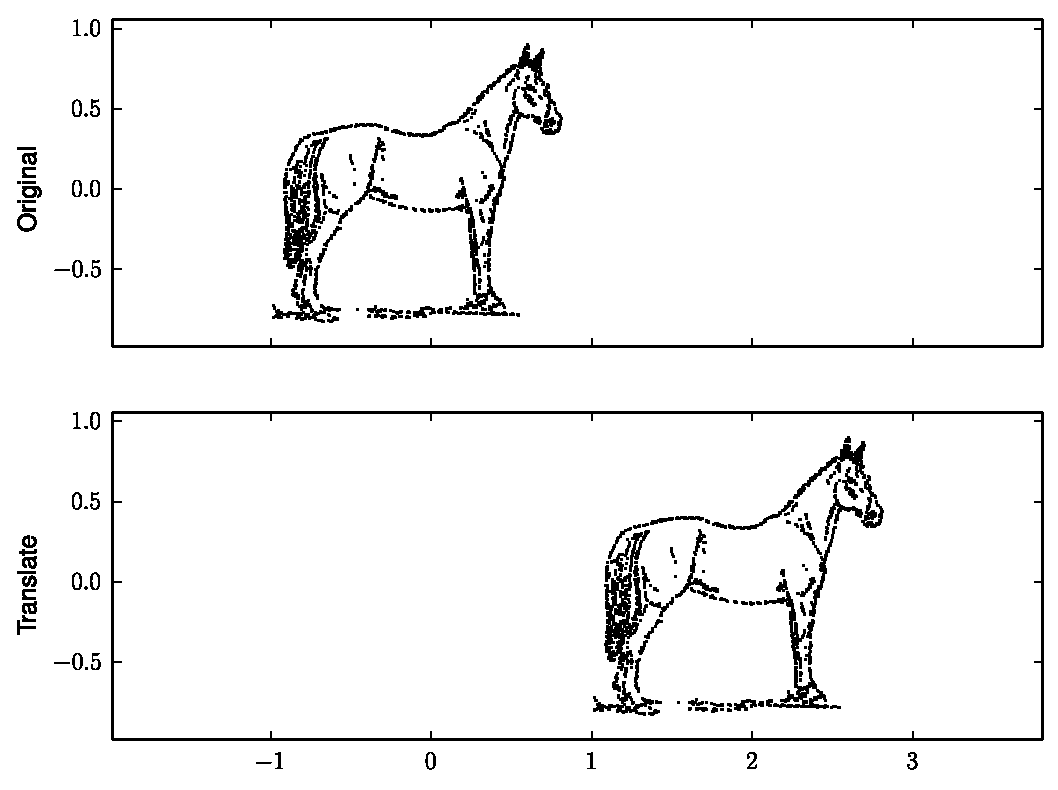
\includegraphics[width=\textwidth]{translate.pdf}
\caption{
An example of a translation.
The top image was translated by the vector $(2, 0)^T$ to produce the bottom image.}
\label{fig:translation}
\end{figure}

A translation is a map $T: \mathbb{R}^2 \rightarrow \mathbb{R}^2$ defined by $T(\mathbf{x}) = \mathbf{x}+\mathbf{b}$ where $\mathbf{b} \in \mathbb{R}^2$. 
For example, if $\mathbf{b} = (2, 0)^T$, then applying $T$ to an image will shift it left by 2. 
This translation is illustrated in Figure \ref{fig:translation}.


Translations are usually NOT linear maps. 
Therefore, they cannot be represented as matrix multiplication.

\begin{problem}
Write a function that accepts an array of points and an array indicating how much to shift them in each direction. 
The function should return the translated points. 
Hint: You can construct a $2 \times 1$ array using the syntax \li{np.array([[a], [b]])}. 
This may be more convenient for broadcasting. 
Another hint: To check your work, plot the original points and their images under the transformation using the function \li{plotOldNew()} defined in Problem \ref{prob:dilation}.
\end{problem}

\subsection*{Affine transformations}
Translations, together, with linear transformations, make up the broader class of transformations called ``affine transformations." 
These are transformations of the form $T: \mathbb{R}^2 \to \mathbb{R}^2$, $T(X) = AX + b$ where $A$ is an $n\times n$ matrix and $b \in \mathbb{R}^n$. 
Affine transformations include all compositions of scalings, rotations, dilations, reflections, and translations. 
For example, if $S$ represents a shear and $R$ a rotation, and if $\mathbf{b}$ is a vector in $\mathbb{R}^2$, then $T(\mathbf{x}) = RS\mathbf{x} + \mathbf{b}$ first shears $\mathbf{x}$, then rotates it, and finally translates it by $\mathbf{b}$. 


\begin{problem}
Imagine a particle $p_1$ rotating around a second particle $p_2$ which is moving through $\mathbb{R}^2$ in a straight line. 
Suppose $p_2$ begins at the origin and $p_1$ begins at $(1, 0)$. 
We can compute the trajectory of $p_1$ using affine transformations.

\begin{enumerate}\label{prob:trajectory}
\item Write a function that returns the position of $p_1$ at a time $t$. 
Your function should accept a time $t$, an angular velocity $\omega$, a direction vector $\mathbf{v}$, and a speed $s$. 
Assume $p_1$ rotates with angular velocity $\omega$ and $p_2$ moves in the direction of $\mathbf{v}$ with speed $s$.
The location of $p_1$ at time $t$ can be computed as follows:
\begin{itemize}
\item Calculate the position of $p_2$ at time $t$ with the formula $(st/\|\mathbf{v}\|) \mathbf{v}$.
\item Calculate the position of $p_1$ as follows:
\begin{itemize}
\item Rotate $p_1$ by $t\omega$ radians.
\item Translate the resulting vector by the vector equal to the position of $p_2$ at time $t$.
\end{itemize}
\end{itemize}
\end{enumerate}
\item Plot the trajectory of $p_1$ on the time interval $(0, 10)$ assuming $\omega=\pi$, $v=(1, 1)$, and $s=3$. 
Your graph should look something like Figure \ref{fig:trajectory}.
\begin{figure}[H]
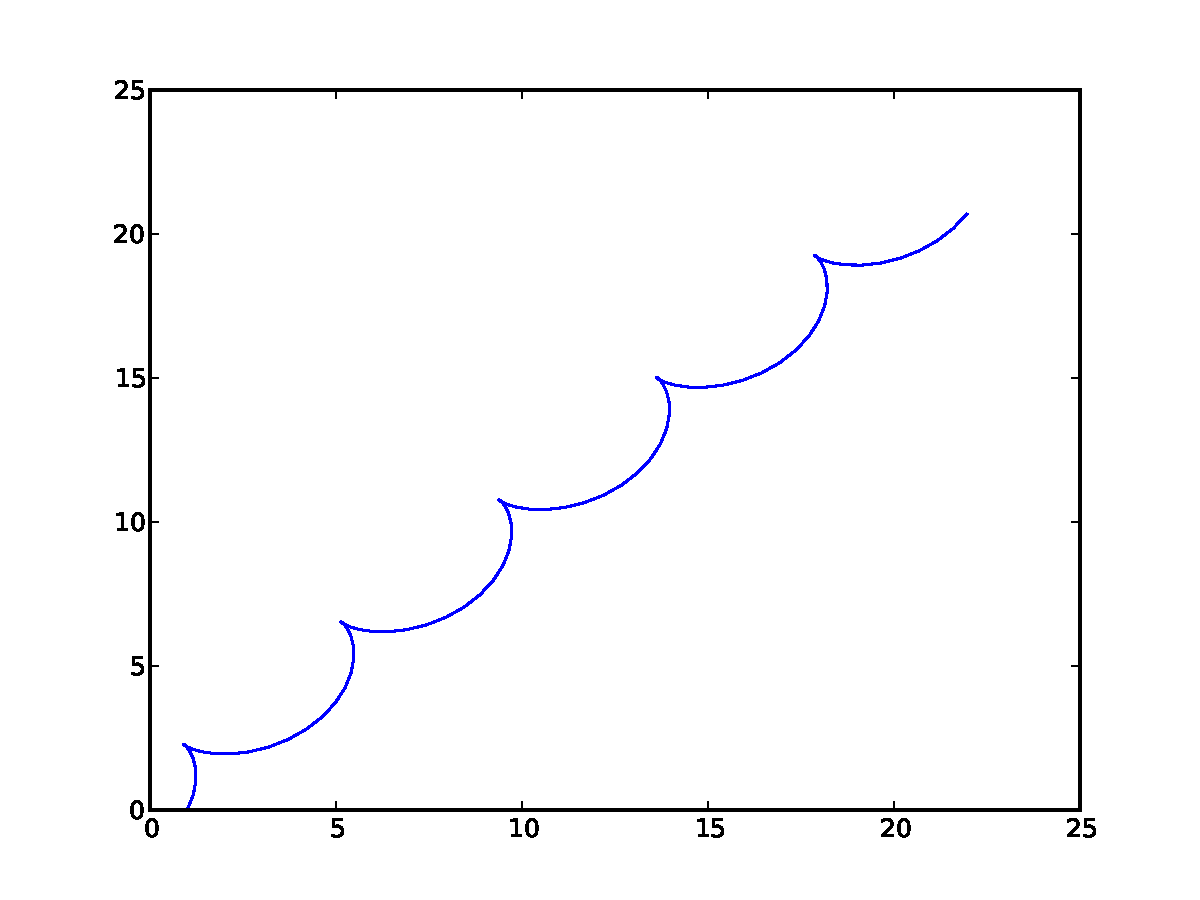
\includegraphics[width=\textwidth]{trajectory.pdf}
\caption{Solution to Problem \ref{prob:trajectory}.}
\label{fig:trajectory} 
\end{figure}
\end{problem}

\section*{Linear systems}
This section describes efficient algorithms for solving systems of linear equations.

\subsection*{Programming elementry row operations}
When you perform a row operation on a matrix, you are really left-multiplying by some elementary matrix. 
However, matrix multiplication is not the most efficient way to implement row operations. It is much faster to perform row operations by modifying the array in place, and only changing those entries that are affected by the operation. 
The following code implements the three elementary row operations by modifying the array in place.

\lstinputlisting[style=fromfile]{row_opers.py}

\subsection*{Programming row reduction}
When you solve a linear system by reducing the matrix with row operations, it is most efficient to reduce only to row echelon form (REF)
\footnote{We do not require leading coefficients to be 1 in the REF.} 
and then use back substitution. 
Here is some code that reduces a matrix to REF.

\begin{lstlisting}
>>> A = np.array([[4., 5., 6., 3.],[2., 4., 6., 4.],[7., 8., 0., 5.]])
array([[ 4.,  5.,  6.,  3.],
       [ 2.,  4.,  6.,  4.],
       [ 7.,  8.,  0.,  5.]])
>>> A[1] -= (A[1,0]/A[0,0]) * A[0]
>>> A[2] -= (A[2,0]/A[0,0]) * A[0]
>>> A[2,1:] -= (A[2,1]/A[1,1]) * A[1,1:]
>>> A
array([[ 4. ,  5. ,  6. ,  3. ],
       [ 0. ,  1.5,  3. ,  2.5],
       [ 0. ,  0. , -9. ,  1. ]])
\end{lstlisting}

In the third row operation modified only a part of the third row because we knew that the first value would still be 0. 
Modifying only those entries of the array that are affected by a row operation will save a lot of time when you are row reducing a large matrix.

Beware that round-off error in row reduction can cause serious problems.
Suppose we wish to row reduce a matrix $A$ as follows.

\begin{lstlisting}
>>> A = np.array([[4., 5., 6., 3.],[2., 2.5, 6., 4.],[7., 8., 0., 5.]])
array([[ 4.,  5.,  6.,  3.],
       [ 2.,  2.5,  6.,  4.],
       [ 7.,  8.,  0.,  5.]])
>>> A[1] -= (A[1,0]/A[0,0]) * A[0]
>>> A[2] -= (A[2,0]/A[0,0]) * A[0]
\end{lstlisting}

If we work this out by hand, at this point we have

\begin{equation}\label{equ:correct_ans}
A = \begin{pmatrix}
4&5&6&3 \\
0&0&3&2.5 \\
0&-7.5&-10.5&-.25
\end{pmatrix}.
\end{equation}

If we swap the second and third rows, then the matrix is in row echelon form. 
However, suppose that due to round-off error, the machine instead computes

\[
A = \begin{pmatrix}
4&5&6&3 \\
0&10^{-15}&3&2.5 \\
0&-7.5&-10.5&-.25
\end{pmatrix}.
\]

The algorithm would then attempt to pivot on the \li{A[1,1]} entry as follows.

\begin{lstlisting}
>>> A[2,1:] -= (A[2,1]/A[1,1]) * A[1,1:]
>>> A
array([[ 4. ,  5.0e+00 , 6.00e+00 ,  3.000e-00 ],
       [ 0. ,  1.0e-14 , 3.00e+00 ,  2.500e-00 ],
       [ 0. ,  0.0e+00 , 2.25e+14 ,  1.875e+14 ]])
\end{lstlisting}

The round-off error in the \li{A[1,1]} entry has affected the third row, and the matrix is now much different than the correct answer in (\ref{equ:correct_ans}). 
In larger matrices, round-off error can propagate through many steps in a calculation, resulting in garbage output.

Some of NumPy's matrix algorithms use row reduction. 
NumPy's methods use several clever tricks to minimize the impact of round-off errors. 
However, these methods may still give you garbage output due to round-off error, especially if the matrix is \emph{ill-conditioned}. 
You should always be aware of this possibility.

\begin{problem}
\label{prob:REF}
Write a function which reduces a square matrix to REF. 
You may make the following assumptions:
\begin{enumerate}
\item The matrix is invertible.
\item During your row reduction, a zero will never appear on the main diagonal.
\item All round-off errors may be ignored.
\end{enumerate}
During a row operation, do not modify any entries that you know will be zero before and after the operation.
\end{problem}

\subsection*{The LU decomposition}
The LU decomposition of a square matrix $A$ is a factorization $A=LU$ where $U$ is an upper triangular and $L$ is a lower triangular matrix. 
In fact, $U$ is the REF of $A$ and $L$ is a product of Type III elementary matrices whose inverses reduce $A$ to $U$. 
Thus, the LU decomposition is a way of storing the REF and ``how we got there.''

The LU factorization of $A$ exists only when $A$ can be reduced to REF using only Type III elementary matrices (no row swaps). 
However, we can always permute the rows of $A$ to obtain a matrix that has an LU decomposition. 
If $P$ encodes the row swaps, then a decomposition $PA = LU$ always exists. 

If $A$ has an LU decomposition (not requiring row swaps), then we can find it as follows. 
Reduce $A$ to REF with $k$ row operations, corresponding to matrices $E_1, \ldots, E_k$. 
Then $U = E_k \ldots E_2E_1A,$ where $U$ is the REF of $A$. 
Because there were no row swaps, each $E_i$ is a lower triangular Type III matrix. Then $E_i^{-1}$ is also lower triangular. 
Thus, $L=(E_k \ldots E_2E_1)^{-1}$ is lower triangular, and $LU=A.$

Because $L=(E_k \ldots E_2E_1)^{-1} = IE_1^{-1}E_2^{-1}\ldots E_k^{-1}$, we can compute $L$ by right-multiplying the identity by the matrices we used to reduce $U$. 
In fact, in this special situation, each right-multiplication will change only one entry of $L$. 
We have the following algorithm for the LU decomposition, assuming it exists.

\begin{itemize}
\item Make a copy, $U$, of $A$.
\item Make an identity matrix $L$ that is the same shape as $A$.
\item Iterate through the entries below the diagonal of $U$.

Now for each entry below the main diagonal of $U$ do the following:
	\begin{itemize}
	\item Set the corresponding entry of $L$ to the quotient of the current entry of $U$ and the entry of the main diagonal of $U$ located above the current entry.
	\item Perform the type 3 row operation to set the current entry of $U$ to 0.
		Do not modify any entries known to be 0.
	\end{itemize}
\item Return $L$ and $U$
\end{itemize}

\begin{algorithm}
\begin{algorithmic}[1]
\Procedure{LU Decomposition}{$A$}
\State $U \gets \text{copy} \left( A \right)$
\State $L \gets I_n$
\For{$0 \leq i < n$}
    \State $R_{i,i} \gets \norm{Q_{:,i}}$
    \State $Q_{:,i} \gets Q_{:,i}/R_{i,i}$
    \For{$i+1 \leq j < n$}
        \State $R_{i,j} \gets Q_{:,j}^\mathsf{T}Q_{:,i}$
        \State $Q_{:,j} \gets Q_{:,j}-R_{i,j}Q_{:,i}$
	\EndFor
\EndFor
\State \pseudoli{return} $Q, R$
\EndProcedure
\end{algorithmic}
\caption{The modified Gram-Schmidt. This algorithm returns orthogonal $Q$ and upper triangular $R$ such that $A = QR$.}
\label{Alg:gram_schmidt}
\end{algorithm}

\begin{problem}
\label{prob:LU_copy}
Write a function that finds the LU decomposition of a square matrix. 
You may assume that the matrix has an LU decomposition.
\end{problem}

The LU decomposition can be performed in-place by storing $U$ on and above the main diagonal of the array and storing $L$ below it.
The main diagonal of $L$ does not need to be stored since all its entries are ones.


\begin{problem}[Optional]
Modify your solution to Problem \ref{prob:LU_copy} so that the function computes the LU decomposition in place.
\end{problem}



\subsection*{Applications of the LU decomposition}
The LU decomposition is a more efficient way to solve linear systems than row reduction, and it can also be used to quickly compute inverses and determinants. 
SciPy implements these methods in the \li{linalg} module, specifically in the functions \li{linalg.lu_factor}, \li{linalg.solve}, \li{linalg.inv}, and \li{linalg.det}.

Let us see how to use the LU decomposition to solve matrix equations. 
Suppose that after row swaps, $A$ has the decomposition $PA = LU$. 
Then $Ax=b$ is equivalent to $LUx=Pb$. 
We can solve this system by first solving $Ly = Pb$ and then $Ux = y$. 
Since $L$ and $U$ are triangular, these systems can be solved with backward and forward substitution, which is faster than row reduction. 
Thus, we can perform row reduction once to compute the $LU$ factorization of $A$, and then we can use substitution to solve $Ax=b$ many different values of $b$. 
This technique is significantly faster than storing $A^{-1}$ and then computing $A^{-1}b$ (see Problem \ref{prob:solve}).

\begin{problem}\label{prob:solve}
In this problem you will solve the system $Ax = b$ for fixed $A$ and many different values of $b$. 
You will do this in two ways. 
For a random $1000 \times 1000$ array $A$ and a random $1000 \times 500$ array $B$ do the following.
\begin{enumerate}
\item Time \li{la.lu_factor(A)}.
\item Time \li{la.inv(A)}.
\item Store the output of \li{la.lu_factor()}. Time \li{la.lu_solve()} on this stored output and $B$.
\item Store the inverse of $A$. Time how long it takes to multiply $A^{-1}$ by $B$.
\item What can you conclude about the more efficient way to solve linear systems?
\end{enumerate}
\end{problem}


Our technique for solving linear equations can also be used to invert matrices. 
We can compute $A^{-1}$ by solving $LUx_i = P_i$ for every $P_i$ that is a column of $P$. 
Then $A^{-1}$ is the matrix with columns $x_1, x_2, \ldots, x_n$. 

Finally, the LU decomposition also gives us an efficient way to compute determinants. 
For if $PA=LU$, then $\det(A) = [\det(P)]^{-1}\det(L)\det(U)$. 
But the determinant of a triangular matrix is the product of its diagonal entries, and every diagonal entry of $L$ is 1. 
Also, $\det(P)$ is the number of row swaps we applied to $A$ to put it in the appropriate form. 
So if $U$ has diagonal entries $u_{ii}$ for $i=1, \ldots, n$, then

\[
\det(A) = (-1)^S\left(\displaystyle\prod_{i=1}^nu_{ii}\right),
\]

where $S$ is the number of row-swaps.



%\begin{problem}
%\label{prob:lusolve}
%Write a function that takes the LU decomposition computed by the second function you made in Problem \ref{prob:LU} and another array representing the right hand side of a linear system and modifies the second array in place so that it represents the solution to the linear system.
%No changes to the array storing the LU decomposition are necessary.
%\end{problem}
%

\begin{problem}[Optional]
\label{prob:det}
Write a function that finds the determinant of a matrix using \li{la.lu_factor()} and the algorithm described above. 
Read the documentation to learn about the output of \li{la.lu_factor()}.
Hint: If the $i^{th}$ entry of the output \li{piv} does not equal $i$, this means that a row swap occurred.
\end{problem}

\subsection*{The Cholesky decomposition (Optional)}
The Cholesky decomposition requires half the calculations and memory of the LU decomposition. 
Furthermore, it is \emph{numerically stable}, which means that round-off errors do not propagate throughout the computation. 
Because of its efficiency and numerical stability, the Cholesky decomposition is used to solve least squares, optimization, and state estimation problems.

However, the Cholesky decomposition is only applicable to Hermitian positive definite matrices. 
A matrix $A$ is positive definite if  $\mathbf{z}^TA\mathbf{z} > 0$ for all $\mathbf{z} \neq 0$. 
Furthermore, $A$ is Hermitian if $A = A^*$ where $A^* = \overline{A^T}$, so a real Hermitian matrix is just a symmetric matrix. 
The Cholesky decomposition is the matrix equivalent to taking the square root of a positive real number.

The Cholesky decomposition of a $A$ is a lower-triangular matrix $L$ such that

\begin{equation*}
 A = LL^*.
\end{equation*}

The entries of $L$ are calculated as follows.

\begin{align*}
&L_{i,j} = \frac{1}{L_{j,j}}\left(A_{i,j} -\sum_{k=1}^{j-1}{L_{i,k}L_{j,k}}\right) \mbox{ for $i>j$} \\ \\
&L_{i,i} = \sqrt{A_{i,i} - \sum_{k=1}^{i-1}{L_{i,k}L_{i,k}}}.
\end{align*}

Notice that the entries of $L$ are defined recursively, with dependencies as diagrammed in Figure \ref{fig:cholesky}. 
Thus, an implementation of the Cholesky decomposition must compute the entries of $L$ in the correct order.

\begin{figure}
\begin{tikzpicture}[red dot/.style={draw, circle, fill=red, red},
	norm/.style={draw=none}, xscale=1.5, yscale=1.5]

\begin{scope}[shift={(4,0)}]
\draw [-,ultra thick](-.2,0)--(-.2,2.5);
\draw [-,ultra thick](2.7,0)--(2.7,2.5);
\draw [-,ultra thick](-.2,0)--(0,0);
\draw [-,ultra thick](-.2,2.5)--(0,2.5);
\draw [-,ultra thick](2.7,2.5)--(2.5,2.5);
\draw [-,ultra thick](2.7,0)--(2.5,0);

\node[norm,black](bk1)at(.25,2.25){\LARGE \textbullet};
\node[norm,black](bk2)at(.75,1.75){\LARGE \textbullet};
\node[norm,black!25!](b1)at(1.25,1.25){\LARGE \textbullet};
\node[norm,black](bk3)at(1.75,.75){\LARGE \textbullet};
\node[norm, black](bk4)at(2.25,.25){\LARGE \textbullet};
\node[norm, black!25!](b2)at(.25,1.25){\LARGE \textbullet};
\node[norm,black!25!](b3)at(.75,1.25){\LARGE \textbullet};
\node[norm,black!25!](b4)at(.25,.25){\LARGE \textbullet};
\node[norm,black!25!](b3)at(.75,.25){\LARGE \textbullet};
\node[norm, shadecolor](r1)at(1.25,.25){\Huge \textbullet};

\end{scope}

\begin{scope}
\draw [-,ultra thick](-.2,0)--(-.2,2.5);
\draw [-,ultra thick](2.7,0)--(2.7,2.5);
\draw [-,ultra thick](-.2,0)--(0,0);
\draw [-,ultra thick](-.2,2.5)--(0,2.5);
\draw [-,ultra thick](2.7,2.5)--(2.5,2.5);
\draw [-,ultra thick](2.7,0)--(2.5,0);


\node[norm, shadecolor](r1)at(1.75,.75){\Huge \textbullet};
\node[norm,black](bk1)at(.25,2.25){\LARGE \textbullet};
\node[norm,black](bk2)at(1.25,1.25){\LARGE \textbullet};
\node[norm,black](bk3)at(.75,1.75){\LARGE \textbullet};
\node[norm,black](bk4)at(2.25,.25){\LARGE \textbullet};
\node[norm,black!25!](bk1)at(.25,.75){\LARGE \textbullet};
\node[norm,black!25!](bk1)at(.75,.75){\LARGE \textbullet};
\node[norm, black!25!](bk1)at(1.25,.75){\LARGE \textbullet};
\end{scope}
\end{tikzpicture}
\label{fig:cholesky}
\caption{The entries of $L$ in the Cholesky decomposition are defined recursively, as illustrated in this picture. 
To calculate the green entry, you need to know each of the light gray entries.}
\end{figure}


\begin{problem}[Optional]
Write a function that finds the Cholesky decomposition of a Hermitian positive definite matrix.
Hint: To generate symmetric positive definite matrices on which to test your function, recall that for any matrix $A$, the matrix $A^TA$ is symmetric and positive definite.
\end{problem}

The \li{linalg} module of SciPy includes an optimized Cholesky decomposition. 
As with the LU decomposition, SciPy has the methods \li{la.cho_factor} and \li{la.cho_solve}.

\begin{problem}[Optional]
Repeat problem \ref{prob:solve}, this time using the methods \li{la.cho_factor} and \li{la.cho_solve}.
\end{problem} 
